\documentclass[12pt]{article}
\usepackage{hyperref}
\usepackage{graphicx}
\usepackage{subcaption}
\begin{document}
\section{Short Answer}


-H-$\alpha$, H-$\beta$ lines etc. are the result of emission/absorption from electrons transitioning between different energy levels of the hydrogen atom. As stars are predominantly made up of hydrogen, we use the existence of the hydrogen spectral lines to verify if the spectrum is from a star. \\
- The strength of the lines is related to the surface temperature of the star. The same star at different temperatures will record a different wavelength for the location of the peak, as well as different flux (and so different EW) values. The surface temperature can be dohetermined by Wien's law, i.e.
T = $ \frac{2.9*10^7}{\lambda_{peak}} $. Furthermore, in general, denser stars have thinner peaks due to the smaller number of collisions that happen. The effect of temperature on the EW is still dominant, however. Also, the strength of a line is proportional to the relative abundance of that element inside the star.

\subsection{ Other absorption lines: (Fig. 1) }
\begin{figure}
\includegraphics[width=16cm]{../otherpeaks}
\caption{Alternative peaks - on the left are peaks at 3836$\AA$ (H-eta), 3890$\AA$ (He-I), 3934$\AA$ (K) and 3970$\AA$ (H), where H and K are Ionized Calcium.   On the right, peaks at 5582$\AA$ (not certain, but I believe this is Titanium Oxide) and at 6306$\AA$ (O-I). I used this source from UChicago to identify the emission lines: \url{http://astro.uchicago.edu/~subbarao/newWeb/line.html}}
\end{figure}
\begin{figure}
\includegraphics[width=16cm]{../otherpeakszoom}\\
\caption{This is a zoomed-in version of Fig. 1, to see the peaks at the lower wavelengths more clearly.}
\end{figure}
\begin{figure}
\includegraphics[width=16cm]{../anotherpeaks}\\
\caption{This is another spectra to show the same peaks appearing for another star.}
\end{figure}

\section{SDSS Data query}
\subsection{ Using the sqlcl.py module within Python to query the SDSS database (DR9)}
- This seeks the standard (calibration) stars as defined on SDSS's "Algorithms" webpage: \url{http://www.sdss3.org/dr9/algorithms/boss_std_ts.php}. \\
- There is one modification: instead of \\ $\sqrt{((u-g)-0.82)^2+((g-r)-0.3)^2+((r-i)-0.09)^2+((i-z)-0.02)^2}<0.08$ we used $|(u-g)-0.82|<0.08$, $|(g-r)-0.3|<0.08$ etc. \\
- The output gives the extinction (in the g-band), the recorded flux, equivalent width and continuum values given in galSpecLine for the H-$\alpha$, H-$\beta$, H-$\gamma$, H-$\delta$ lines. \\
- However, due to the reported equivalent widths being unreasonable compared to manual estimations, the query also extracts the plate-mjd-fiber values and downloads, via wget, the relevant FITS file for this plate-mjd-fiber combination. \\
- The full query is here: 
\begin{verbatim}"SELECT p.objID, p.extinction_g, s.elodieTEff, p.extinction_g,
 p.extinction_g, p.extinction_g, p.extinction_g, p.extinction_g,
 p.obj, s.plate, s.fiberID, s.mjd, g.h_alpha_flux, g.h_alpha_reqw, 
 p.psfMag_u, p.psfMag_g, p.psfMag_r, p.psfMag_i, p.psfMag_z 
    FROM PhotoObj AS p 
    JOIN SpecObj as s ON s.specobjID=p.specobjID 
    WHERE psfMag_r BETWEEN 15.0 and 19.0 
    AND p.type=6 AND  dbo.fPhotoStatus('PRIMARY')>0 AND 
dbo.fPhotoFlags('STATIONARY')>0  and  calibStatus_r=1 
AND s.elodieTEff!=0 AND s.elodieFeH!=0 AND s.elodieLogG!=0 
 AND  ((flags&dbo.fPhotoFlags('BLENDED')) 
 +(flags&dbo.fPhotoFlags('DEBLEND_TOO_MANY_PEAKS')) +   
(flags&dbo.fPhotoFlags('SATURATED')) +
(flags&dbo.fPhotoFlags('BADSKY')) + 
(flags&dbo.fPhotoFlags('COSMIC_RAY')) +
(flags&dbo.fPhotoFlags('PEAKS_TOO_CLOSE')) +   
(flags&dbo.fPhotoFlags('NOTCHECKED_CENTER')) +
(flags&dbo.fPhotoFlags('SATUR_CENTER')) +  
(flags&dbo.fPhotoFlags('INTERP_CENTER')) +
(flags&dbo.fPhotoFlags('INTERP'))+  
(flags&dbo.fPhotoFlags('PSF_FLUX_INTERP')))=0 
    AND  (psfMag_u-psfmag_g) between 0.82-0.08 and 0.82+0.08 
    AND (psfMag_g-psfmag_r) between 0.3-0.08 and 0.30+0.08 
    AND (psfMag_r-psfmag_i) between 0.09-0.08 and 0.09+0.08 
    AND (psfMag_i-psfmag_z) between 0.02-0.08 and 0.02+0.08 
    ORDER BY extinction_g DESC"\\
\end{verbatim}
\section{Redshift correction}
- The wavelengths were corrected for redshift using the value recorded from HDU2 (copy of SpecObj table from SDSS)\\
\begin{figure}
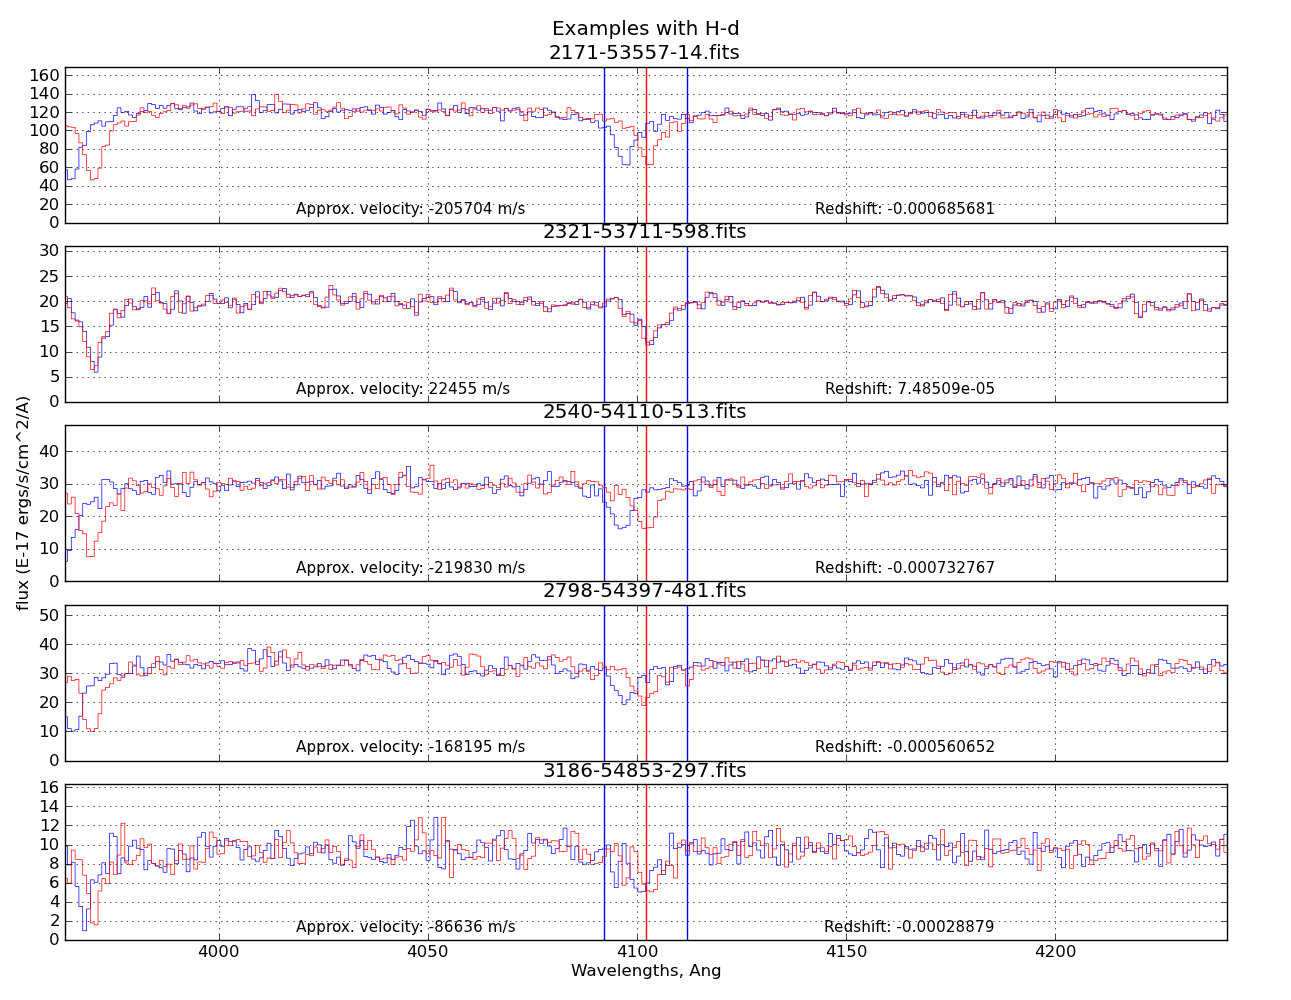
\includegraphics[width=8cm]{../splines_correct}\\
\caption{Red line shows redshift correction; blue shows the reversed correction.}
\end{figure}

\begin{figure}
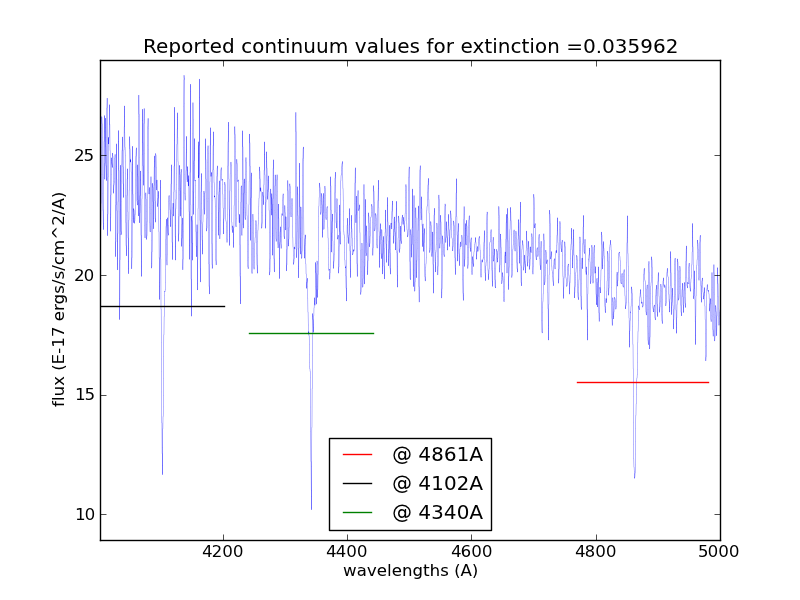
\includegraphics[width=8cm]{../035}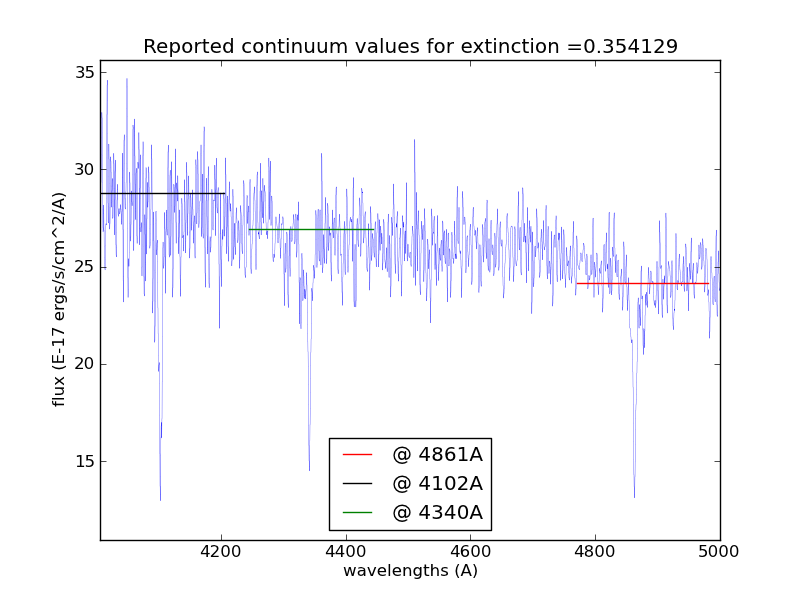
\includegraphics[width=8cm]{../355}\\
\caption{The recorded continuum values in GalSpecLine seem to be only valid for high (above 0.25) extinction values.}
\end{figure}
\section{Working with Equivalent Widths}
\subsection{Generating the new continuum, flux and equivalent width values}
- The equivalent width is defined by the width such that the area of a rectangle with a height of the continuum value is equal to the area in a spectral line.\\
- We want to use equivalent widths because they essentially measure flux in units of continuum. This means it gives the fraction of light absorbed, instead of the actual number of photons. This means that even if two stars are of different brightness, if viewed through the same interstellar medium (e.g. dust) they will have similar equivalent widths. Moreover, the equivalent width is independent of instrumental resolution and so allows for low-resolution spectra to be used.\\
- However, the calibration of the spectra is suspect - the atmosphere might be introducing unknown wavelength-dependent multiplicative factors, so new values need to be generated using the SDSS spectra.\\
- The spectra are first corrected for redshift.\\
- A cubic spline is used to interpolate the spectrum over a common rest-wavelength grid.\\
- Near the location of each peak, a neighborhood of $\pm$100$\AA$ is taken, excluding a $\pm$10$\AA$ neighborhood (which will be used for flux integration) and the median of this is taken as the continuum, and a $\pm$10$\AA$ neighborhood is taken as the domain for the flux integration.\\
- The flux is numerically integrated over this 20$\AA$ range, using the trapezium rule, and the ratio of flux/continuum gives the equivalent width value.\\
- The [continuum, flux, equivalent width, peak location] is taken for a given peak (e.g. H-$\beta$) for each spectra and collected into one array; then this is repeated for all the absorption lines used and collected into one array. This array can be stored in a binary text file using the "pickle" function. \\
\begin{figure}
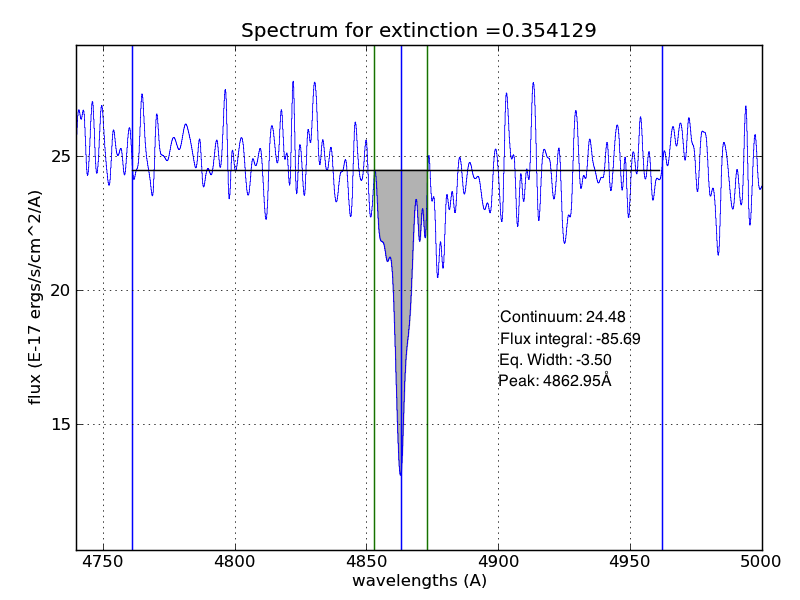
\includegraphics[width=8cm]{../workingexample}\\
\caption{This shows the continuum and equivalent-width estimation. The green lines are each 10$\AA$  away from the central blue line. The blue lines in the extreme left and right are defined at 4761$\AA$ and 4962$\AA$  respectively. The shaded gray area is the flux and the black horizontal line is the continuum.}
\end{figure}
\subsection{Changing the filters to determine the significance of each color filter in the number of stars}
- Each of the (u-g), (g-r), (r-i) and (i-z) filters was changed individiually from 0.08 to 0.20 in graduations of 0.005, while holding the other three constant at 0.08. 
- It was found that (u-g) and (g-r) were most important for increasing the number of stars; each of these filters was linearly proportional to the number of stars returned by the SQL query, while the (r-i) and (i-z) filters quickly tapered off. 

\begin{figure}
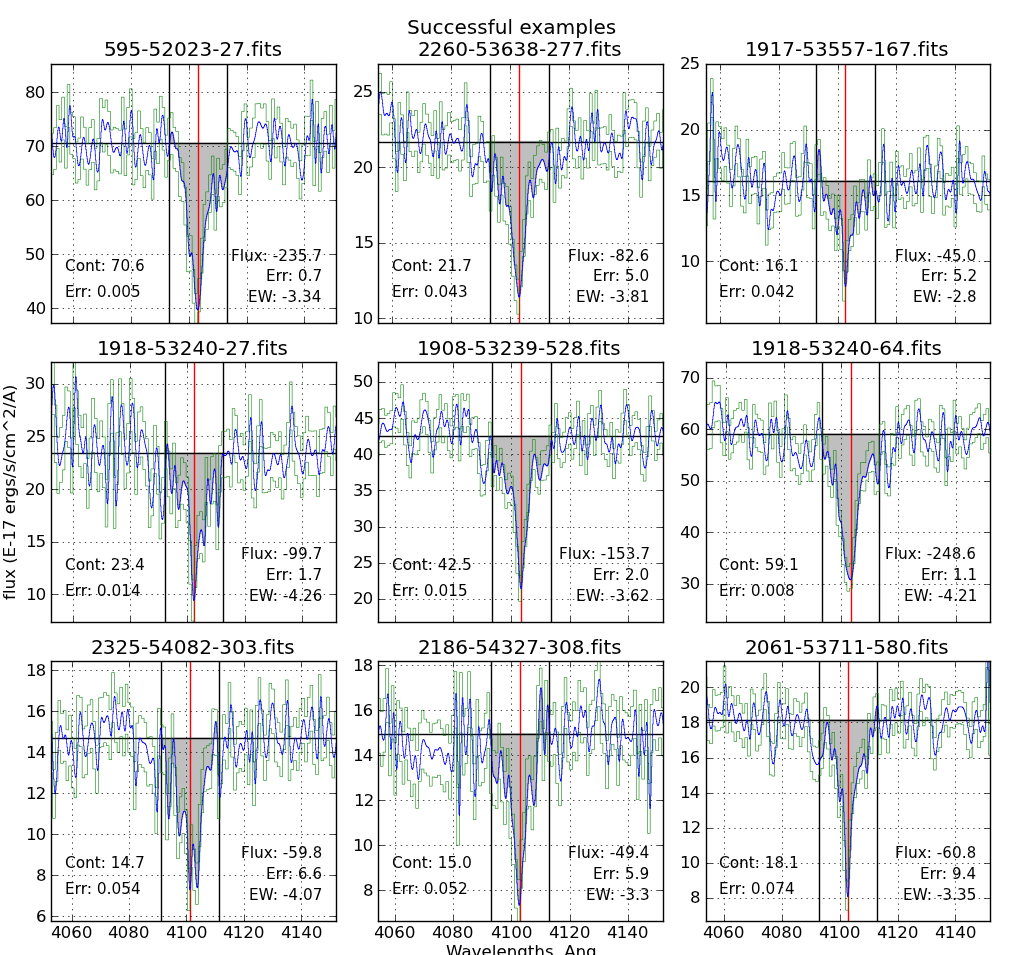
\includegraphics[width=10cm]{../success_labeled}\\
\caption{Example calculations for spectra.}
\end{figure}

\begin{figure}
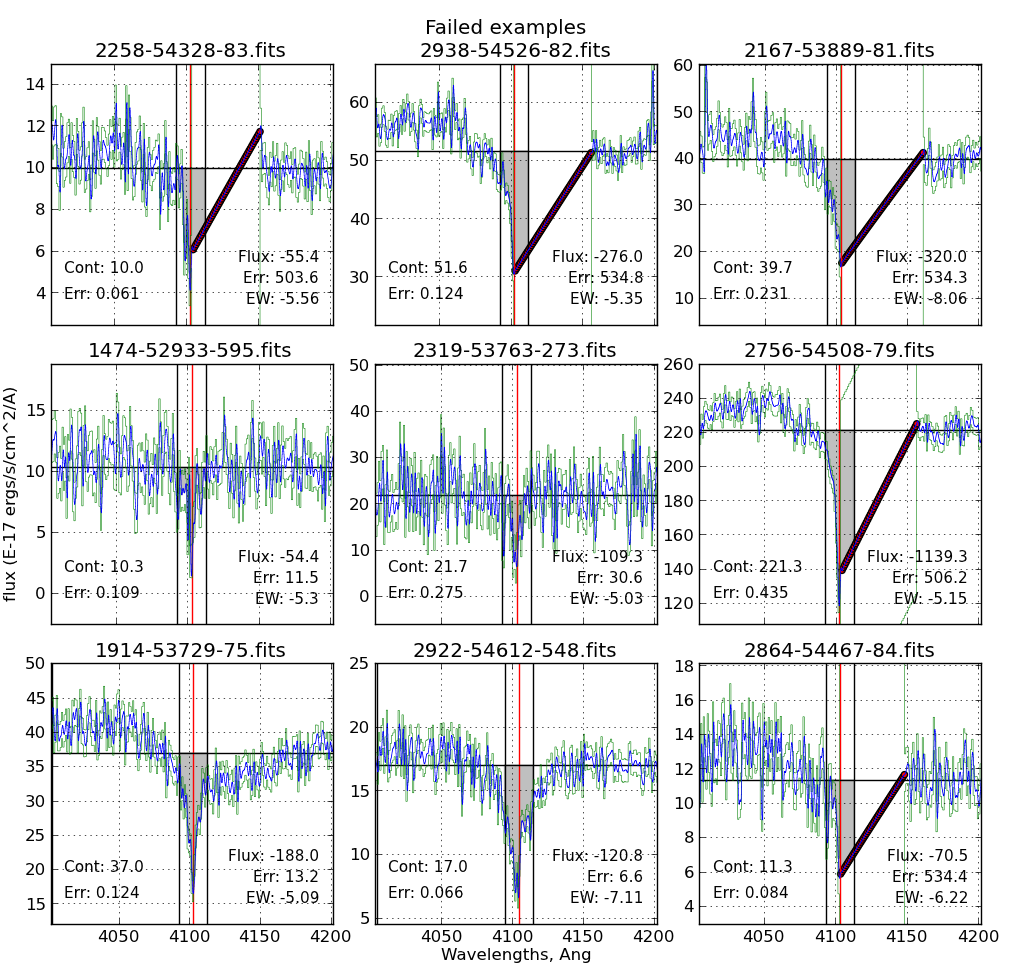
\includegraphics[width=8cm]{../failb_labeled}\\
\caption{Noted failures: varying reasons lead to an overestimate of the flux and consequentially, equivalent width. The main sources are (1) a sudden jump in flux values; (2) a particularly noisy spectrum which leads to a lot of flux from the wings being included; (3) the continuum being not very flat which means more there is more flux between the continuum line and spectrum.}
\end{figure}
\begin{figure}
\includegraphics[width=6cm]{../varyingug}\includegraphics[width=6cm]{../varyi-z}\\
\caption{ On the left, the linear relationship of u-g vs number of stars can be seen, and on the right the nonlinear relationship of r-i vs number of stars can be seen.}
\end{figure}
\subsection{Finding relationship between u-g and g-r; triangle.py module}
- A scatterplot was made of g-r vs u-g to see if there was a correlation between g-r and u-g. 
\begin{figure}
\includegraphics[width=8cm]{../ug&gr2}\\
\caption{A scatter plot of g-r vs u-g; however, it is not clear what the distribution is like, although the there does seem to be a correlation.}
\end{figure}
- The same parameters were taken and with the \href{https://github.com/dfm/triangle.py}{triangle.py module} a corner plot was made, which shows the contours.\\
\begin{figure}
\includegraphics[width=8cm]{../triangle}\\
\caption{The corner plot, expanded to also include the i-z filter, showing the pairwise distribution of these three filters.}
\end{figure}
\begin{figure}
\includegraphics[width=8cm]{../h_bgd_tri}\\
\caption{A corner plot with H-$\alpha$, H-$\beta$ and H-$\gamma$ with color filter 0.08.}
\end{figure}
\begin{figure}
\includegraphics[width=8cm]{../hdbg_expandb}\\
\caption{A corner plot with H-$\alpha$, H-$\beta$ and H-$\gamma$ with color filter 0.16. Points with error greater than the flux integral are excluded (this therefore excludes all points with ivar=0 in any of the equivalent width calculations.}
\end{figure}
\begin{figure}
\includegraphics[width=8cm]{../hd_tscat_ext_tri}\\
\caption{A corner plot with H-$\delta$, extinction in the g band and the recorded effective temperature from the SDSS database with color filter = 0.08. Because the temperatures in the database are rounded to the nearest 500K or so, a random number between -100 and 100 was added to each point to improve scatter.}
\end{figure}
\begin{figure}
\includegraphics[width=8cm]{../HdTeffExtgExpand}\\
\caption{A corner plot with H-$\delta$, extinction in the g band and the recorded effective temperature from the SDSS database with color filter = 0.16. A random number between -100 and 100 was added to each point to improve scatter.} 
\end{figure}
\begin{figure}
\includegraphics[width=12cm]{../newAllLineEWall_notlog}\\
\caption{A corner plot with all equivalent widths of all lines, including those flagged as having infinite error.} 
\end{figure}
\begin{figure}
\includegraphics[width=12cm]{../newAllLineEWgood_notlog}\\
\caption{A corner plot with equivalent widths of all lines where the continuum and flux errors were finite.} 
\end{figure}
\subsection{Testing out Linear Discriminant Analysis module for future use}
- The LDA module from \href{http://scikit-learn.org/stable/install.html}{scikit-learn} was installed.
- It was tested on the u-g vs g-r plot from above, with the two classes chosen randomly by the objID, so there is no statistical significance in the below plot.\\
\begin{figure}
\includegraphics[width=6cm]{../LDAtest}\\
\caption{Test application of LDA module to show potential usage. The two classes are color-coded and the boundary line is plotted. The module also allows for Quadratic Discriminant Analysis (not shown).}
\end{figure}


\section{Errors}
- The ivar entry was used from the HDU 2 of each fits file: when the ivar was not zero, standard error =  $\frac{1}{\sqrt{ivar}}$. If the ivar was zero, the standard error was set as 100. \\
- The continuum estimation error is estimated using a linear combination of the standard errors divided by the number of values used to compute the continuum. The fluxes with ivar=0 are not used in the calculation for the continuum and these errors are therefore not included in the continuum estimation error.\\
$Error_{cont} = \frac{\sqrt{\sigma_1^2 + ... + \sigma_i^2 + ... + \sigma_n^2}}{n}$\\
- The flux estimation error is estimated using a linear combination of the standard errors, treating the trapezium rule as a linear combination. The fluxes with ivar=0 are used in the calculation of the flux and so integrals that include these flux values will have significantly higher errors.\\
$Error_{flux} = h\sqrt{1\sigma_1^2+4\sigma_2^2+ ... + 4\sigma_i^2 + ... + 4\sigma_{n-1}^2+1\sigma_n^2}$, where h is the step size used in the trapezium approximation\\
\begin{figure}
\begin{subfigure}{.5\textwidth}
\includegraphics[width=6cm]{../Logcont_err_good_org}
\caption{With only points having error$\textless$continuum value.}
\end{subfigure}
\begin{subfigure}{.4\textwidth}
\includegraphics[width=6cm]{../Logcont_err_all_org}
\caption{With all points.}
\end{subfigure}
\caption{Log-log graphs of continuum value vs continuum error, using r=0.08}
\end{figure}
\begin{figure}
\begin{subfigure}{.5\textwidth}
\includegraphics[width=6cm]{../Logcont_err_good_exp}
\caption{With only points having error$\textless$continuum value.}
\end{subfigure}
\begin{subfigure}{.4\textwidth}
\includegraphics[width=6cm]{../Logcont_err_all_exp}
\caption{With all points.}
\end{subfigure}
\caption{Log-log graphs of continuum value vs continuum error, using r=0.16}
\end{figure}
\begin{figure}
\begin{subfigure}{.5\textwidth}
\includegraphics[width=6cm]{../Logflux_err_good_org}
\caption{With only points having error$\textless$flux value.}
\end{subfigure}
\begin{subfigure}{.4\textwidth}
\includegraphics[width=6cm]{../Logflux_err_all_org}
\caption{With all points.}
\end{subfigure}
\caption{Log-log graphs of flux value vs flux error, using r=0.08}
\end{figure}
\begin{figure}
\begin{subfigure}{.5\textwidth}
\includegraphics[width=6cm]{../Logflux_err_good_exp}
\caption{With only points having error$\textless$flux value.}
\end{subfigure}
\begin{subfigure}{.4\textwidth}
\includegraphics[width=6cm]{../Logflux_err_all_exp}
\caption{With all points.}
\end{subfigure}
\caption{Log-log graphs of flux value vs flux error, using r=0.16}
\end{figure}


\section{Computational time}
- The number of queries returned using the SQL query above is 5204, taking a few minutes to run. To download all these FITS files takes approximately 3 hours. To assemble all the flux/wavelength data into an array for computing the EW, then computing the EW and relevant errors takes approximately 1 hour. \\
- If the filter range is increased from $\pm$0.08 to $\pm$0.16, the query returns 17452 stars. This includes the 5204 stars from the original query, and as these FITS files do not need to be re-downloaded, the remaining 12248 FITS files require 6 hours to download.\\
- As each FITS file is approximately 500KB-2MB in size, a typical computer can only process 2000-3000 FITS files at a time due to memory constraints. Even if the FITS files are closed again, Python does not reallocate the memory and the garbage-collection module did not help either. As a result, it is best to do the EW computation in blocks of 2000-3000, and to save each array each time as a binary text file, then to load it again and append the next block onto it.\\
- Each block of 2700 takes around 30 minutes to append the FITS files and compute the EW.


\section{Ratios of spectra; sorted via EW and extinction}
- The 7541 stars returned by the SQL query using DR8 were processed using the above EW calculation method.\\
- They were sorted by EW and 9 quantiles were taken, each containing 754 stars: between the 5th-15th percentiles, 15th-25th etc. all the way up to 85th-95th.\\
- Then each quantile was sorted by extinction, and again 9 quantiles, each containing 75 stars, were taken between the 5th-15th percentiles, 15th-25th, etc. all the way up to 85th-95th percentile in extinction.\\
- This yields 81 quantiles, each containing 75 stars, sorted by extinction after sorting for EW.\\
- For each quantile, all the fluxes corresponding to wavelengths between 3900A and 8000A were taken and everything else was discarded: this meant that all the measurements had a common wavelength array.\\
- The "average spectrum", consisting of averaging the total flux measured at each of the wavelength measurements, was plotted. This was sorted by EW, i.e. for each EW quantile, 9 plots were made corresponding to each extinction quantile and put into one figure.\\
- For each EW quantile, the average of the 9 plots, i.e. the average of all 754 spectra within that quantile, was calculated. The ratio of each of the 9 plots to this average was plotted.\\
\begin{figure}
\includegraphics[width=12cm]{../spectra_avg_8}\\
\caption{Panel of 9 plots of the average spectra of each extinction quantile, all of one particular EW quantile.}
\end{figure}
\begin{figure}
\includegraphics[width=12cm]{../spectra_avg_ratio_8}\\
\caption{Panel of 9 plots of the ratio of the average spectra of each extinction quantile to the average spectra of all extinction values within one particular EW quantile.}
\end{figure}

\section{Linear Fitting}
- At each particular wavelength, all the flux, H-delta EW, extinction (g), and g-band magnitude were collected. \\
- A linear model was fitted to find three coefficients:\\
observed flux = a$\times$Brightness + b$\times$H-$\delta$ EW + c$\times$Extinction, where brightness 10$^{-0.4 \times (mag_g - 22.5)}$\\
- These coefficients were different for each wavelength, and a plot of each coefficient as a function of wavelength was plotted.\\
\begin{figure}
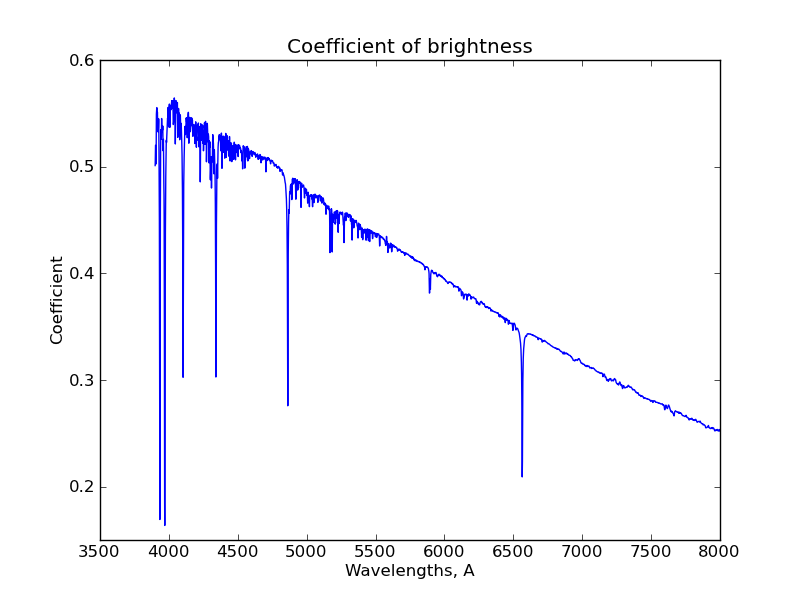
\includegraphics[width=12cm]{../coeffs0}\\
\caption{Coefficients of brightness as a function of wavelength}
\end{figure}
\begin{figure}
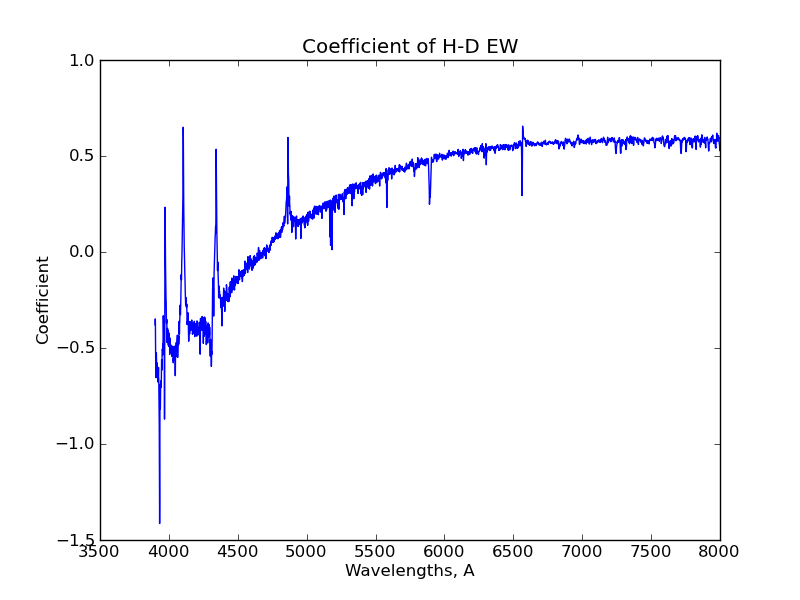
\includegraphics[width=12cm]{../coeffs1}\\
\caption{Coefficients of H-$\delta$ as a function of wavelength}
\end{figure}
\begin{figure}
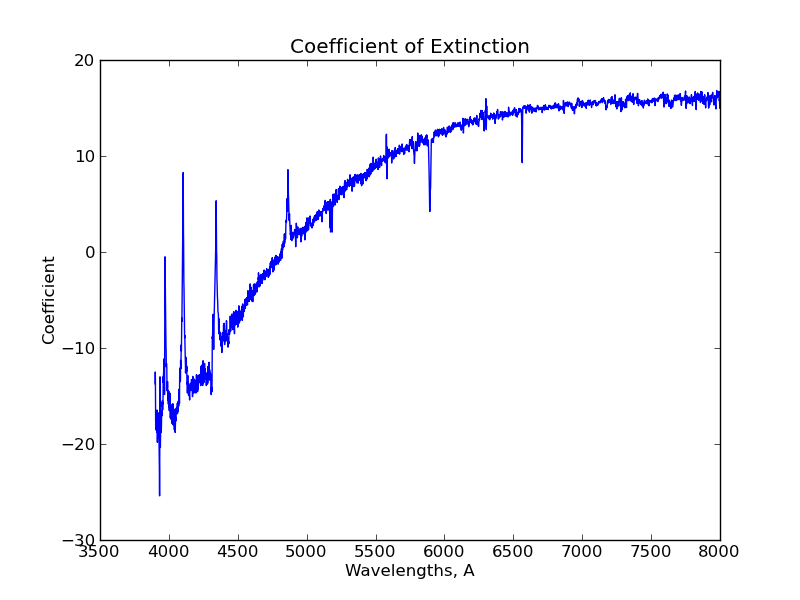
\includegraphics[width=12cm]{../coeffs2}\\
\caption{Coefficients of extinction as a function of wavelength}
\end{figure}
\begin{figure}
\begin{subfigure}{.5\textwidth}
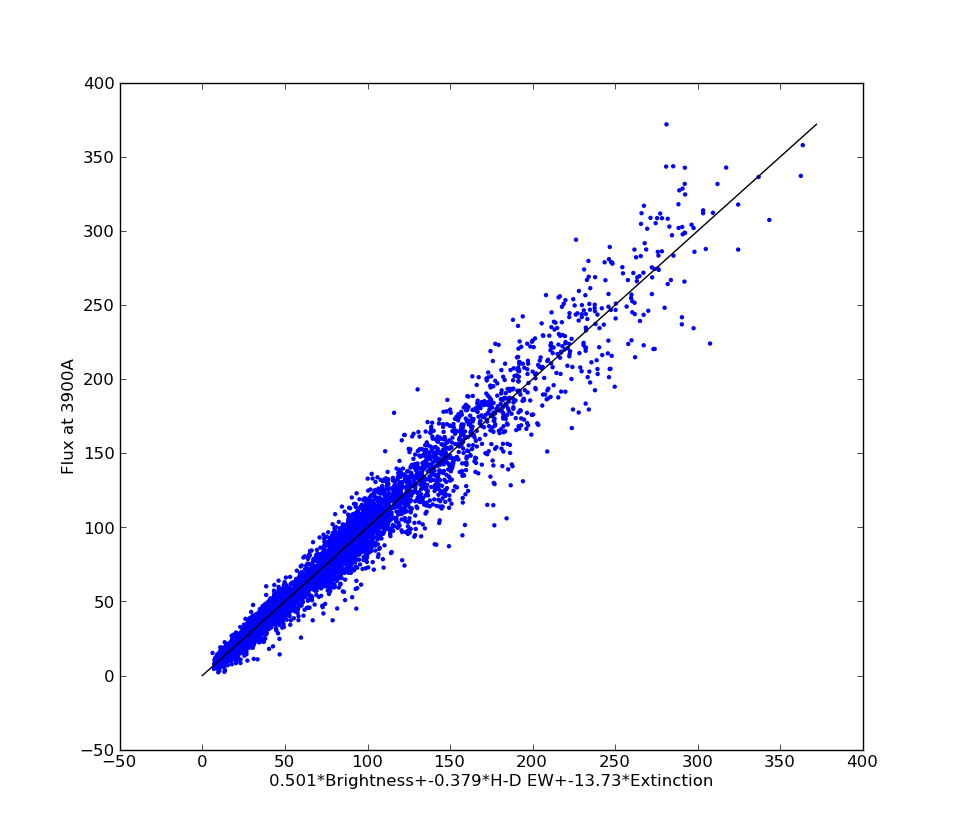
\includegraphics[width=6cm]{../residuals}\\
\caption{Plot of expected flux values using the coefficients, and the actual flux values at 3900$\AA$. The y=x line is plotted to represent a perfect fit.}
\end{subfigure}
\begin{subfigure}{.5\textwidth}
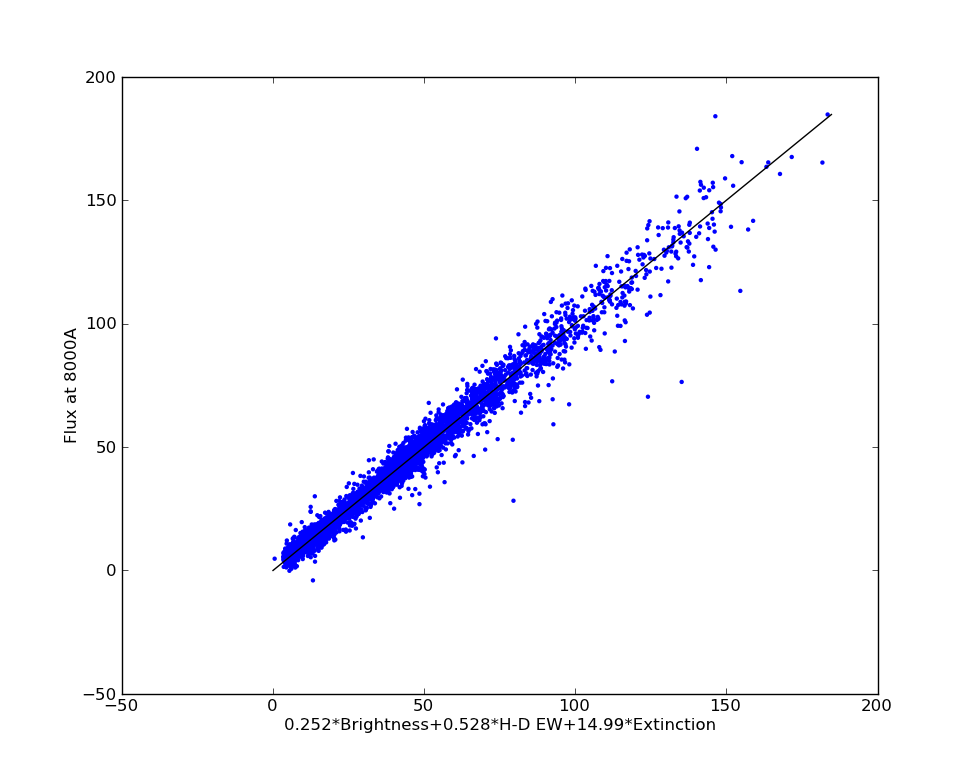
\includegraphics[width=6cm]{../residuals8000}\\
\caption{Plot of expected flux values using the coefficients, and the actual flux values at 8000$\AA$.}
\end{subfigure}
\end{figure}
\end{document}